\documentclass[conference]{IEEEtran}
\usepackage{tikz}
\usetikzlibrary{positioning, arrows.meta, fit, calc}
\usepackage{amsmath}
\usepackage{amssymb}
\usepackage{listings}
\usepackage{xcolor}
\usepackage{booktabs}

\lstset{
  basicstyle=\ttfamily\scriptsize,
  breaklines=true,
  frame=single,
  framerule=0.2pt,
  backgroundcolor=\color{gray!5}
}

\tikzset{
  block/.style={draw, rounded corners=2pt, minimum height=2.2em, minimum width=6em, align=center, font=\scriptsize},
  layer/.style={block, fill=orange!12, minimum width=13em},
  store/.style={block, fill=blue!8},
  human/.style={block, fill=red!10},
  gen/.style={block, fill=green!10},
  state/.style={draw, rounded corners=6pt, minimum height=1.9em, align=center, font=\tiny, fill=gray!8},
  arr/.style={-{Stealth[length=2mm]}, thick},
  darr/.style={arr, dashed},
  lbl/.style={font=\tiny, midway}
}

\title{Mining Legacy Python Corpora into a Provenance-Tracked Automation Platform with Human-in-the-Loop Delivery}

\author{
\IEEEauthorblockN{Johnny~Morgan}
\IEEEauthorblockA{Information Systems, UMBC\\
yj07538@umbc.edu}
}

\begin{document}
\maketitle

\begin{abstract}
Organizations accumulate years of Python code across many projects performing similar but distinct work, leaving substantial capability locked in unindexed scripts. We present a layered platform that converts such a corpus into an automated product-delivery system. Layer~1 crawls the filesystem and catalogs every source file and its documentation---location, project, purpose, description---in a central database. Layer~2 detects repeated code blocks performing the same purpose using three tiers of clone detection (normalized-AST hashing, FAISS similarity over structural n-grams, and semantic adjudication). Layer~3 consolidates clone clusters into library functions published to a private PyPI server, with mandatory database provenance linking every function to the source blocks it replaced. Layer~4 validates the libraries by re-executing original workloads and comparing outputs against golden masters; no script retires unvalidated. Layer~5 exposes a generative interface that resolves customer requests to cataloged capabilities, schedules execution, and routes every product through a human reviewer who approves release or rejects for rework. Requests with no matching capability route to data scientists, whose code onboards through the same pipeline---closing the growth loop. The same machinery drives scheduled periodic reporting. The design's invariants are a single database spine, provenance at every level, validation-gated retirement, and human-gated release.
\end{abstract}

\section{Introduction}
The maintenance reality of long-lived analytical organizations is a filesystem of project directories: hundreds of scripts, written over years, solving overlapping problems in incompatible ways. The cost is threefold---rediscovery is manual, duplication compounds, and every new request restarts near zero. Refactoring wholesale is infeasible; the corpus is too large and its behavior is the only specification that exists.

We treat the corpus itself as the specification. The platform mines it in layers: index, detect duplication, consolidate with provenance, validate against original behavior, then serve requests against the validated catalog. Two properties distinguish the design from generic refactoring tooling: \emph{provenance is never optional} (every library function, job, and delivered product traces to its sources), and \emph{humans gate release} (the generative layer proposes and executes; only a named reviewer releases to a customer).

\section{Design Invariants}
\begin{enumerate}
\item \textbf{The database is the spine.} Nothing is ``known'' to the platform unless it is a row. All six layers read and write one catalog.
\item \textbf{Provenance is mandatory.} Library functions record source blocks; jobs record exact library versions; approvals record the reviewer.
\item \textbf{Nothing retires unvalidated.} An original script is superseded only after Layer~4 proves output equivalence.
\item \textbf{Humans gate release.} No product reaches a customer without an approval row.
\end{enumerate}

\section{Layered Architecture}
Fig.~\ref{fig:layers} shows the pipeline; all layers converge on the catalog.

\begin{figure}[t]
\centering
\resizebox{\columnwidth}{!}{%
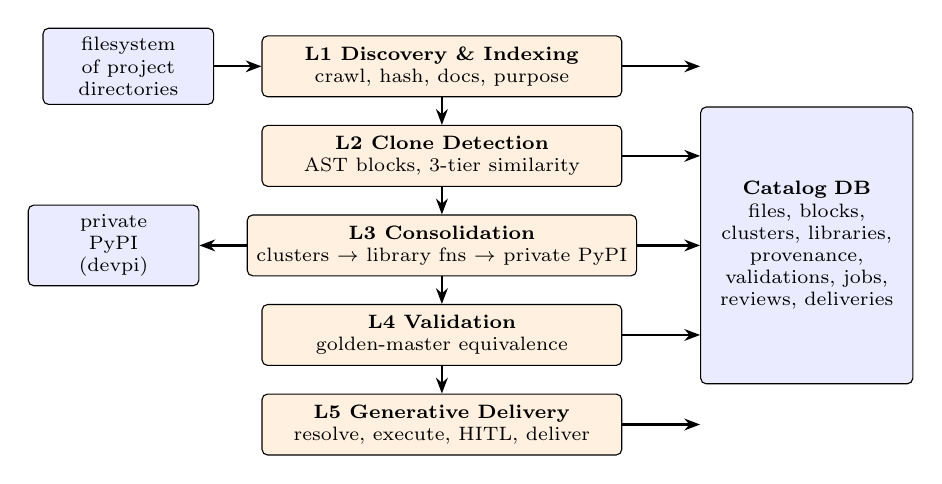
\begin{tikzpicture}[node distance=3.5mm and 8mm]
\node[layer] (l1) {\textbf{L1 Discovery \& Indexing}\\crawl, hash, docs, purpose};
\node[layer, below=of l1] (l2) {\textbf{L2 Clone Detection}\\AST blocks, 3-tier similarity};
\node[layer, below=of l2] (l3) {\textbf{L3 Consolidation}\\clusters $\rightarrow$ library fns $\rightarrow$ private PyPI};
\node[layer, below=of l3] (l4) {\textbf{L4 Validation}\\golden-master equivalence};
\node[layer, below=of l4] (l5) {\textbf{L5 Generative Delivery}\\resolve, execute, HITL, deliver};
\node[store, right=of l3, minimum height=10em, text width=7em] (db) {\textbf{Catalog DB}\\files, blocks,\\clusters, libraries,\\provenance,\\validations, jobs,\\reviews, deliveries};
\draw[arr] (l1) -- (l2);
\draw[arr] (l2) -- (l3);
\draw[arr] (l3) -- (l4);
\draw[arr] (l4) -- (l5);
\draw[arr] (l1.east) -- (db.west |- l1.east);
\draw[arr] (l2.east) -- (db.west |- l2.east);
\draw[arr] (l3.east) -- (db.west |- l3.east);
\draw[arr] (l4.east) -- (db.west |- l4.east);
\draw[arr] (l5.east) -- (db.west |- l5.east);
\node[store, left=6mm of l1, text width=5.5em] (fs) {filesystem\\of project\\directories};
\node[store, left=6mm of l3, text width=5.5em] (pypi) {private\\PyPI\\(devpi)};
\draw[arr] (fs) -- (l1);
\draw[arr] (l3) -- (pypi);
\end{tikzpicture}%
}
\caption{Layered pipeline over a single catalog database. Each layer writes what the next layer reads; the private PyPI server holds consolidated libraries.}
\label{fig:layers}
\end{figure}

\subsection{L1: Corpus Discovery and Indexing}
A crawler walks the directory roots, identifying Python sources, notebooks, and documentation. Each file is recorded with path, inferred project, content hash, imports, and entry points. Purpose and description come from docstrings and READMEs where present; otherwise an LLM summarization pass generates them, flagged as machine-generated so provenance of the description itself is preserved. Indexing is idempotent and incremental, keyed on content hash.

\subsection{L2: Code-Block Analysis}
Files are parsed to ASTs; candidate blocks (functions, methods, statement spans above a minimum size) are extracted with normalized fingerprints. Similarity runs in three tiers of increasing cost, each only over the prior tier's survivors: (T1)~normalized-AST hashing for exact and renamed clones; (T2)~cosine similarity over AST-n-gram vectors in a FAISS index for modified copies; (T3)~code-embedding similarity with LLM adjudication (``do these perform the same purpose?'') for independent reimplementations. Pairwise edges are clustered into clone clusters---the unit of consolidation.

\subsection{L3: Library Consolidation with Provenance}
Clusters are ranked by member count, cross-project spread, and block size; cross-project spread is the strongest signal of a genuine shared capability. For each selected cluster, a canonical signature is designed to parameterize the members' variations; the implementation is LLM-drafted and human-reviewed, packaged, and published to the private PyPI server. Provenance rows map each library function to every source block it subsumes, with notes on which parameter covers which variation. Replacement scripts---originals re-expressed as library calls---enter the catalog as new files linked to what they replace.

\subsection{L4: Behavioral Validation}
For each consolidated script, original outputs on representative inputs are captured as golden masters; original and replacement execute in isolated, dependency-pinned environments on identical inputs. Comparators are type-appropriate: byte equality for deterministic artifacts, tolerances for floats, schema-plus-content for dataframes, seeded statistical comparison for stochastic outputs. A script's \texttt{retired} flag is set only when all its cases pass; failures return to L3 as defect reports.

\subsection{L5: Generative Delivery with HITL Gate}
Fig.~\ref{fig:lifecycle} shows the request lifecycle. The generative model receives a customer request plus retrieval over the catalog and proposes a capability match and execution plan. Plans run as scheduled jobs recording exact library versions---extending provenance to the product level. Completed products enter a review queue carrying the request, plan, provenance chain, and outputs; the reviewer approves (scheduled delivery) or rejects (rework with notes). Below-threshold resolution or absent capability routes the request to a data scientist as a development ticket; delivered code onboards through L1--L4 and only then becomes resolvable capability. Scheduled periodic reports are standing requests on cron triggers using the identical machinery.

\begin{figure}[t]
\centering
\resizebox{\columnwidth}{!}{%
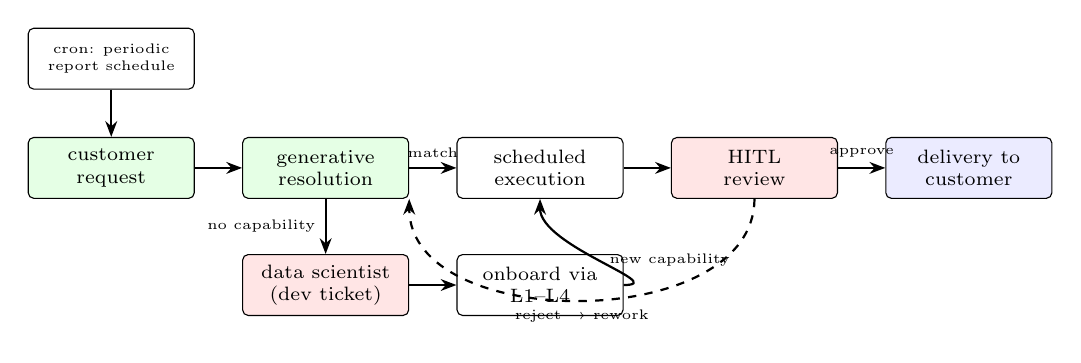
\begin{tikzpicture}[node distance=4mm and 6mm]
\node[gen] (req) {customer\\request};
\node[gen, right=of req] (res) {generative\\resolution};
\node[block, right=of res] (exec) {scheduled\\execution};
\node[human, right=of exec] (rev) {HITL\\review};
\node[store, right=of rev] (del) {delivery to\\customer};
\node[human, below=7mm of res] (ds) {data scientist\\(dev ticket)};
\node[block, right=of ds] (onb) {onboard via\\L1--L4};
\draw[arr] (req) -- (res);
\draw[arr] (res) -- node[lbl, above] {match} (exec);
\draw[arr] (exec) -- (rev);
\draw[arr] (rev) -- node[lbl, above] {approve} (del);
\draw[darr] (rev.south) to[out=-90, in=-90] node[lbl, below] {reject $\rightarrow$ rework} (res.south east);
\draw[arr] (res) -- node[lbl, left] {no capability} (ds);
\draw[arr] (ds) -- (onb);
\draw[arr] (onb.east) to[out=0, in=-90] node[lbl, right] {new capability} (exec.south);
\node[block, above=6mm of req, font=\tiny] (cron) {cron: periodic\\report schedule};
\draw[arr] (cron) -- (req);
\end{tikzpicture}%
}
\caption{Request lifecycle. Every product passes the human gate; capability gaps route to development and re-enter through the mining pipeline itself.}
\label{fig:lifecycle}
\end{figure}

\section{Provenance Chain}
Fig.~\ref{fig:prov} traces a delivered product backward: delivery $\rightarrow$ approving review $\rightarrow$ job with pinned library versions $\rightarrow$ library functions $\rightarrow$ source blocks $\rightarrow$ files $\rightarrow$ projects. Every link is a foreign key; the audit trail is a database query, not an investigation.

\begin{figure}[t]
\centering
\resizebox{\columnwidth}{!}{%
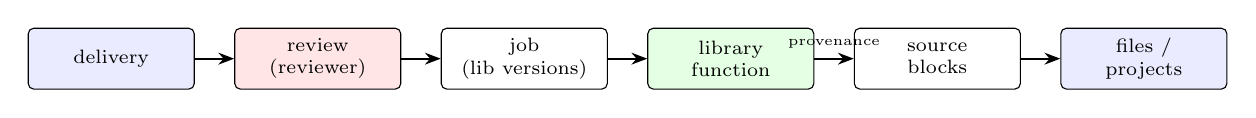
\begin{tikzpicture}[node distance=3mm and 5mm]
\node[store] (dlv) {delivery};
\node[human, right=of dlv] (rv) {review\\(reviewer)};
\node[block, right=of rv] (jb) {job\\(lib versions)};
\node[gen, right=of jb] (lf) {library\\function};
\node[block, right=of lf] (bk) {source\\blocks};
\node[store, right=of bk] (fl) {files /\\projects};
\draw[arr] (dlv) -- (rv);
\draw[arr] (rv) -- (jb);
\draw[arr] (jb) -- (lf);
\draw[arr] (lf) -- node[lbl, above] {provenance} (bk);
\draw[arr] (bk) -- (fl);
\end{tikzpicture}%
}
\caption{Product-to-source provenance chain. Foreign keys at every hop.}
\label{fig:prov}
\end{figure}

\section{Failure Modes and Guards}
\begin{table}[h]
\scriptsize
\centering
\begin{tabular}{p{3.6cm} p{3.9cm}}
\toprule
\textbf{Failure} & \textbf{Guard} \\
\midrule
False clone merge / missed semantic clone & Three-tier detection; LLM adjudication and human review before consolidation \\
Library changes behavior silently & Golden-master gate; retirement only on full pass; defects route to L3 \\
Lost audit trail & Mandatory provenance at function and product level \\
Unreviewed release & Schema-enforced: delivery requires approval row \\
Generative misresolution & Confidence threshold routes to development; reviewer sees plan and provenance \\
Corpus drift & Idempotent incremental re-index; new code enters the same pipeline \\
\bottomrule
\end{tabular}
\end{table}

\section{Discussion}
The platform's growth loop is its most important property: capability gaps do not bypass the architecture, they feed it. New code written for an unmet request is indexed, clone-checked, potentially consolidated, validated, and only then served---so the catalog's guarantees hold uniformly over mined legacy code and freshly written code alike. The corpus stops being an archive and becomes the substrate of a delivery system whose every output is traceable, validated, and human-approved.

\end{document}
